\documentclass[14pt,xcolor=dvipsnames,pdftex]{beamer}
\usepackage[utf8x]{inputenc}
\usepackage[T1]{fontenc}
\usepackage[english]{babel}
\usepackage{hyperref}
\usepackage{pgfpages}
\usepackage{color}
\usepackage{textcomp}
\usepackage{alltt}
\usepackage{amsmath}
\usepackage{amsfonts}
\usepackage{booktabs}
\usepackage{textcomp}
\usepackage{color}

\usepackage{tikz}
\usetikzlibrary{calc,arrows,matrix,fit,positioning}

\usepackage{lmodern}

\newcommand{\tikzmark}[2]{\tikz[overlay,remember picture,baseline=(#1.base)] \node (#1) {#2};}

\usepackage{inconsolata} % TT font
\usepackage{array}
\usepackage{url}
%\usepackage[svgnames]{xcolor}\\
%\usetheme[secheader]{Boadilla}
%\usefonttheme{sans}
\setbeamersize{text margin left=1cm,text margin right=1cm}
\setbeamertemplate{section in toc}[Palo Alto]

\newcolumntype{T}{c<{\ttfamily}}

\title{Phylogenomic inference}
\subtitle{Hauptseminar Frishman WS2013/2014}
\author{Uli Köhler}
\date{February 3rd 2014}

\setbeamertemplate{footline}
{%
%\begin{beamercolorbox}[wd=0.5\textwidth,ht=3ex,dp=1.5ex,leftskip=.5em,rightskip=.5em]{author in head/foot}%
%\usebeamerfont{author in head/foot}%
%\insertframenumber\hfill\insertshortauthor%
%\end{beamercolorbox}%
\vspace*{-4.5ex}\hspace*{0.5\textwidth}%
\begin{beamercolorbox}[width=\textwidth,ht=3ex,dp=1.5ex,left]{title in head/foot}%
\usebeamerfont{title in head/foot}%
Folie \insertframenumber{} von \inserttotalframenumber\hspace{8mm}
%\insertshorttitle%
\end{beamercolorbox}%
}

\AtBeginSection[]{} % for optional outline or other recurrent slide

\begin{document}
\bgroup
\setbeamercolor{background canvas}{bg=black}

\begin{frame}[plain]{}
\end{frame}

\egroup

\frame{\titlepage}

\begin{frame}{Structure of this talk}
\begin{itemize}
\item Issues of non-phylogenic functional prediction
\item What is phylogenomic inference?
\item Phylogenetic tree reconciliation
\item Phylogenomic inference methodology
\item Phylogenomic databases and algorithms:
\begin{itemize}
 \item SIFTER
 \item PhyloFacts
\end{itemize}
\item Common problems of phylogenomic predictions
\item Future of phylogenomics
\item Seminar conclusion
\end{itemize}
\end{frame}

\begin{frame}{Non-phylogenomic function prediction}
 \begin{itemize}
  \item \textit{High-throughput sequencing}\\
  \textrightarrow\ Many proteins, few information available:\\
  \textasciitilde $90000$ PDB structures vs $5.1\times10^6$ UniProt/TrEMBL sequences
  \item Alignment score does not distinguish between matching domains
  \item Difficult to separate \textit{orthologs} and \textit{paralogs}
 \end{itemize}
\end{frame}

\begin{frame}[allowframebreaks]{What is phylogenomic inference?}
 \begin{tikzpicture}[scale=0.65,>=latex',yshift=-3cm]
 \tikzstyle{toptext}=[font=\huge,minimum height=3em,anchor=mid,text centered]
 \tikzstyle{labeltext}=[font=\large,minimum height=3em,anchor=west,text centered]
 \begin{scope}[yshift=-4cm]
  % Text at the top
  \node [toptext,yshift=1mm](phylo) {\raisebox{0pt}[\height][0pt]{\textcolor{ForestGreen}{Phylo}}};
  \node [toptext,right=-3mm of phylo](genomic)
    {\raisebox{0pt}[\height][0pt]{\textcolor{Red}{genomic}}};
  \node [toptext,right=0cm of genomic] (inference)
    {\raisebox{0pt}[\height][0pt]{\textcolor{Blue}{inference}}};
  % Labels
  \node [labeltext,below=4cm of phylo,xshift=4cm] (phylolabel)
      {\textcolor{ForestGreen}{Evolutionary relationship (phylogenetics)}};
  \node [labeltext,below=2.4cm of genomic,xshift=1cm] (genomicslabel)
      {\textcolor{Red}{analyze genomes}};
  \node [labeltext,below=10mm of inference] (inferencelabel)
      {\textcolor{Blue}{infer function}};
  % Arrows
  \draw [thick,->,arrowhead=4mm, line width=2pt]
      (phylolabel.north -| phylo.north) to (phylo);
  \draw [thick,->,arrowhead=4mm, line width=2pt]
      (genomicslabel.north -| genomic.north) to (genomic);
  \draw [thick,->,arrowhead=4mm, line width=2pt]
      (inferencelabel.north -| inference.north) to (inference);
 \end{scope}
 \end{tikzpicture}
 \framebreak
 \begin{itemize}
  \item Concept to enhance homology-based function predictions
  \item Can be applied to both genes and proteins
  \item Attempt to \textbf{separate \textit{orthologs} and \textit{paralogs}}\\
  \textrightarrow\ \textit{ortholog} = high probability of similar or identical function
  \item \textit{Phylogenetic tree reconciliation}:\\
        Identify \textit{speciation} and \textit{duplication} events in phylogenetic trees
 \end{itemize}
\end{frame}

\begin{frame}<1-3>{Tree reconciliation}
\begin{tikzpicture}
\onslide<1->
\tikzset{
  protein/.style = {block, align=center, text centered,fill=orange,
		    draw, rectangle, rounded corners},
  ancestor/.style = {block,minimum size=0cm},
  connection/.style = {thick,draw,arrowhead=4mm, line width=2pt}
};
%Protein nodes
\node [protein] (proteinA) {A};
\node [protein, right=2cm of proteinA] (proteinB) {B};
\node [protein, right=2cm of proteinB] (proteinC) {C};
%Invisible ancestors
\node [ancestor,yshift=2cm] (AB) at ($(proteinA)!0.5!(proteinB)$) {};
\node [ancestor,yshift=3cm] (ABC) at ($(proteinB)!0.5!(proteinC)$) {};
%Paths
\draw [connection]
      (proteinA) |- (AB.east);
\draw [connection]
      (proteinB) |- (AB.west);x
%To-root
\draw [connection]
      ([yshift=1.37mm]ABC.south) -- ([yshift=1.1cm]ABC.north);
%C -> root
\onslide<1-2>
\draw [connection]
      (proteinC) |- (ABC.west);
\draw [connection]
      ([yshift=1.4mm]AB.south) |- (ABC.east);
\onslide<3>
\draw [connection,dashed]
      (proteinC) |- (ABC.west);
\draw [connection]
      ([yshift=1.4mm]AB.south) |- ([xshift=-2mm]ABC.east);
%Text
\onslide<1>
\node [right=5mm of proteinC,text width=3cm,yshift=2cm] (txt)
      {Are B and C \textit{ortholog}\\or \textit{paralog} in respect to A?};
\onslide<2>
\node [left=0mm of ABC,yshift=10mm,x](dupspecLabel){\textcolor{red}{Duplication or speciation?}};
\draw [draw=red,->, line width=2pt]
      (dupspecLabel) to [bend right=15]([yshift=-1mm]AB.mid);
\draw [draw=red,->, line width=2pt]
      (dupspecLabel) to (ABC.mid);
%Slide 3: Example
\onslide<3>
\node [left=2cm of ABC,yshift=15mm](dupspecLabel){(Example)};
\node [left=5mm of AB,yshift=10mm](specLabel){\textcolor{ForestGreen}{Speciation}};
\node [right=1cm of ABC,yshift=5mm](dupLabel){\textcolor{Red}{Duplication}};
\draw [draw=ForestGreen,->, line width=2pt]
      (specLabel) to ([yshift=-1mm]AB.mid);
\draw [draw=red,->,line width=2pt]
      (dupLabel) to ([yshift=-1mm]ABC.mid);

\node [right=5mm of proteinC,text width=3cm,yshift=2cm] (txt)
      {B: \textit{ortholog}\\C: \textit{paralog}};
\end{tikzpicture}
\end{frame}

\begin{frame}[allowframebreaks]{Phylogenomic inference methodology}
 \begin{enumerate}
  \item Cluster homolog proteins
  \item Compute multiple alignment
  \item Edit alignment (remove potential non-homologs)
  \item Mask less-conserved regions in alignment
  \item Construct phylogenetic tree
  \item Identify closely related subtrees
  \item Overlay with experimental data
  \item Differentiate \textit{orthologs} and \textit{paralogs}\\
	(\textit{Tree reconciliation})
  \item Infer function from \textit{orthologs}
 \end{enumerate}
 \framebreak
 \begin{enumerate}
   \item \textcolor{gray}{Cluster homolog proteins}
   \item \textcolor{gray}{Compute multiple alignment}
   \item \textcolor{gray}{Edit alignment}
   \item \textcolor{gray}{Mask less-conserved regions in alignment}
 \end{enumerate}
 \begin{itemize}
  \item Raw alignments would introduce noise
  \item Retain only high-scoring homology \& highly-conserved domains
 \end{itemize}
 %%%%%
 \framebreak
 \begin{enumerate}
  \setcounter{enumi}{4}
  \item \textcolor{gray}{Construct phylogenetic tree}
 \end{enumerate}
 \begin{itemize}
  \item Core problems:
  \begin{itemize}
   \item No information about actual ancestors is available
   \item High computational complexity (optimal solution: NP-Hard!)
  \end{itemize}
  \item Use algorithms like \textit{maximum parsimony} or \textit{maximum likelihood}
 \end{itemize}
 %%%%%
 \framebreak
 \begin{enumerate}
  \setcounter{enumi}{5}
  \item \textcolor{gray}{Identify closely related subtrees}
  \item \textcolor{gray}{Overlay with experimental data}
 \end{enumerate}
 \begin{itemize}
  \item More filtering to reduce noise
  \item Given the tree topology, use only closely related subgroups (in addition to filtering distant homologs in step 1)
 \end{itemize}
 %%%%%
 \framebreak
 \begin{enumerate}
  \setcounter{enumi}{7}
  \item \textcolor{gray}{Differentiate \textit{orthologs} and \textit{paralogs}}
 \end{enumerate}
 \begin{itemize}
  \item Computational tree reconciliation -- examples:
  \begin{itemize}
  \item NCBI COG DB: Bidirectional top BLAST hits
  \item Complex statistical algorithms like RIO (\textit{Resampled inference of orthologs}), \textit{orthostrapper} or \textit{BETE}
  \end{itemize}
  \item Computationally intensive, requires highly-filtered input data
 \end{itemize}
\end{frame}

\begin{frame}{SIFTER}
 \begin{enumerate}
  \setcounter{enumi}{8}
  \item \textcolor{gray}{Infer function from \textit{orthologs}}
 \end{enumerate}
\begin{itemize}
 \item \textit{Statistical Inference of Function Through Evolutionary Relationships}
 \item Predicts protein function (homology-based) given a reconciled tree\\
 \textrightarrow\ Tree construction \& reconciliation remains a problem
 \item Based on bayesian statistics
 \item Complex mathematics (not shown here)
\end{itemize}
\end{frame}

\begin{frame}[allowframebreaks]{PhyloFacts}
 \begin{itemize}
  \item \glqq Encyclopedia\grqq of \glqq books\grqq for known protein (super)families and structura domains
  \item 92800 families (as of 2013-02-03)
  \item Precomputed phylogenetic trees \& phylogenomic family HMMs\\
  \textrightarrow\ Reasonably fast, but\\\glqq\textit{Some results can take hours to complete}\grqq
  \item Provides structured access to annotated phylogenomic information about protein (super)families
 \end{itemize}
 %%%%
 \framebreak
 \begin{columns}[T]
 \begin{column}{.7\textwidth}
 \begin{itemize}
  \item \textbf{FAT-CAT}: PhyloFacts Webservice to predict protein function using phylogenomic methods
  \item Integrates with \textit{Pfam} and uses HMMs to find the sequence position in the precomputed tree
 \end{itemize}
 \end{column}
  \begin{column}{.3\textwidth}
   
\includegraphics[width=1.2\textwidth]{figures/fatcat.jpg}
  \end{column}
 \end{columns}
 \framebreak
 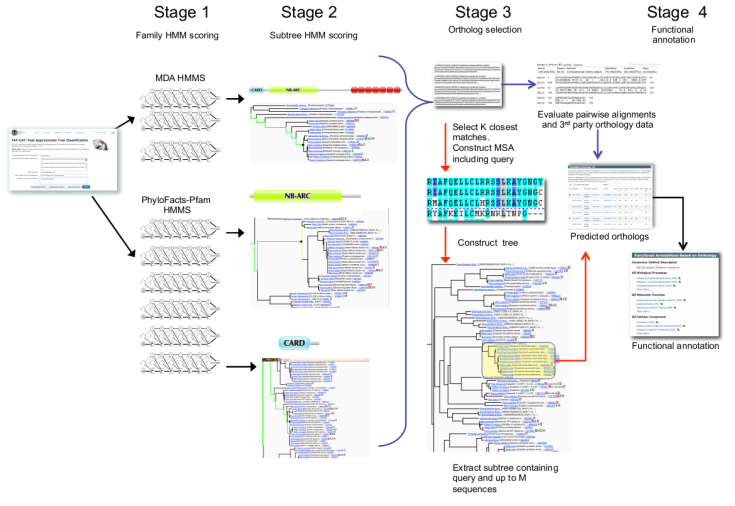
\includegraphics[width=\textwidth]{figures/fatcat-pipeline.png}
\end{frame}

\begin{frame}[allowframebreaks]{Issues of phylogenomic methods}
  \textcolor{ForestGreen}{\textit{in-silico}}\ --\ \textcolor{Red}{Involves manual steps}
 \begin{enumerate}
  \item \textcolor{Red}{Cluster homolog proteins}
  \item \textcolor{ForestGreen}{Compute multiple alignment}
  \item \textcolor{Red}{Edit alignment}
  \item \textcolor{Red}{Mask less-conserved regions in alignment}
  \item \textcolor{ForestGreen}{Construct phylogenetic tree}
  \item \textcolor{ForestGreen}{Identify closely related subtrees}
  \item \textcolor{Red}{Overlay with experimental data}
  \item \textcolor{ForestGreen}{Differentiate \textit{orthologs} and \textit{paralogs}}
  \item \textcolor{Red}{Infer function from \textit{orthologs}}
 \end{enumerate}
 %%%%
 \framebreak
 \begin{enumerate}
  \item \textcolor{gray}{Cluster homolog proteins}
  \item \textcolor{gray}{Compute multiple alignment}
  \item \textcolor{gray}{Edit alignment}
  \item \textcolor{gray}{Mask less-conserved regions in alignment}
  \end{enumerate}
  \begin{itemize}
   \item Manual annotation \& selection\\
   \textrightarrow\ Subjective, error-prone, time/cost-intensive
   \item Information will be lost, does the annotator just select what he wants to see?
   \item Algorithms too sensitive, are results always reliable?
  \end{itemize}
 %%%
 \framebreak
 \begin{enumerate}
  \setcounter{enumi}{4}
  \item \textcolor{gray}{Construct phylogenetic tree}
 \end{enumerate}
 \begin{itemize}
  \item \textit{Distance-based} vs. \textit{character-based} construction algorithms
  \item Small, highly-conserved protein families perform better than large (super)families
  \item Lack of consistency across methods
  \item Algorithms scale poorly
  \textrightarrow\ Can't be used for large (super)families
  \item Some methods produce millions of equivalently scored topologies
 \end{itemize}
 %%%
 \framebreak
 \begin{enumerate}
  \setcounter{enumi}{6}
  \item \textcolor{gray}{Overlay with experimental data}
 \end{enumerate}
 \begin{itemize}
  \item Database = Experimental data + sinferred data
  \item Experimental datasets available
        $\leftrightarrow$ Protein function already know
  \item Protein function unknown $\leftrightarrow$ few experimental datasets available
 \end{itemize}
 %%%
 \framebreak
 \begin{itemize}
  \item Multiple subsequent filter passes
  \item Huge sets of parameters, impossible to select optimal values
  \item Requires manual annotation \& experimental data
  \item S	ometimes even \textit{orthology} is not sufficient for annotation transfer
  \item Doesn't work well with distant homologs, requires highly-conserved domains
  \end{itemize}
\end{frame}

\begin{frame}{Future of phylogenomic inference}
 \begin{itemize}
  \item Phylogenomics alone has too many problems and open questions, but...
  \pause
  \item ...\textbf{together with other concepts} functional prediction accuracy can be enhanced
  \item Computational complexity: Moore's law and alternative computational hardware\\
  \textrightarrow\ Large-scale application feasible in the future?
  \item Phylogenomic inference for DB verification
  \item Can also be applied to other attributes (besides protein function)
  \item PhyloFacts \& SIFTER: Usable tools, but apparently not widely adopted or actively developed
 \end{itemize}
\end{frame}

\begin{frame}{Conclusion (Phylogenomic inference)}
 \begin{itemize}
  \item Powerful concept for enhancing function prediction accuracy by identifying \textit{orthologs}
  \pause
  \item ... if it would actually work in practice
  \item Too complex, too manual, too many parameters
  \item Pure \textit{in-silico} phylogenomics\\
  \textrightarrow\ Low quality results
  \item Manual annotation can't keep up with \textit{HTS}
  \item PhyloFacts provides a useful database for function prediction using phylogenomic approaches
 \end{itemize}
\end{frame}

\begin{frame}{Conclusion (Seminar)}
\begin{itemize}
\item \textit{in-silico} protein function inference is a yet unsolved problem in computational biology
\item Combine any information that is available, including:
\begin{itemize}
 \item Context-based prediction
 \item Alternative splicing
 \item SNPs
 \item Phylogenomics
 \item Experimental results
\end{itemize}
\item \textbf{Only with all this information combined sufficient accurracy for \textit{in-silico} function prediction is achievable}
\end{itemize}
\end{frame}

\begin{frame}
  \frametitle<presentation>{References}    
  \begin{thebibliography}{10}
  \tiny
  \beamertemplatearticlebibitems
  \bibitem{}
    Kimmen~Sjölander
    \newblock Phylogenomic inference of protein molecular function: advances and challenges
    \newblock {\em Bioinformatics}, 2004
  %\beamertemplatearticlebibitems
  \bibitem{}
    Barbara~E.~Engelhardt et al.
    \newblock Protein Molecular Function Prediction by Bayesian Phylogenomics
    \newblock {\em PLoS Computational Biology}, 2005
  %\beamertemplatearticlebibitems
  \bibitem{}
    Jonathan~A.~Eisen \& Claire~M.~Frasier
    \newblock Phylogenomics:Intersection of Evolution and Genomics
    \newblock {\em Science}, 2003
  %\beamertemplatearticlebibitems
  \bibitem{}
    Duncan~Brown, Kimmen~Sjölander
    \newblock Functional Classification using Phylogenomic Inference
    \newblock {\em PLoS Computational Biology}, 2006
  %\beamertemplatearticlebibitems
  \bibitem{}
    Nandini Krishnamurthy et al.
    \newblock PhyloFacts: an online structural phylogenomic encyclopedia for protein functional and structural classification
    \newblock {\em Genome Biology}, 2006
  %\beamertemplatearticlebibitems
  \bibitem{}
    Barbara~E.~Engelhardt et al.
    \newblock A graphical model for predicting protein molecular function
    \newblock {\em Proceedings of the International Conference on Machine Learning (ICML)}, 2006
  \end{thebibliography}
\end{frame}

\begin{frame}
 \begin{center}
 {\color{BlueViolet}\large Thank you for your attention!}\\[1cm]
 {\small References and sources available at}\\
 {\small \url{https://github.com/ulikoehler/Hauptseminar}}\\[1cm]
 {\color{BlueViolet}\large Questions?}\\[1cm]
 \end{center}
\end{frame}

\end{document}